\ifsvnmulti
 \svnkwsave{$RepoFile: lyapunov/dailyBlog.tex $}
 \svnidlong {$HeadURL$}
 {$LastChangedDate$}
 {$LastChangedRevision$} {$LastChangedBy$}
 \svnid{$Id$}
\fi

\chapter{Daily blog}
\label{c-DailyBlog}

\begin{bartlett}{
Je ne veux pas travailler\\
Je ne veux pas dejeuner\\
Je veux seulement oublier\\
Et puis je fume
            }
\bauthor{
\HREF{http://www.youtube.com/watch?v=MBoTRF2aK4s}
{China Forbes - Thomas M. Lauderdale (Pink Martini)}
    }
\end{bartlett}

\renewcommand{\ssp}{x}
\renewcommand{\vel}{\ensuremath{v}}   % state space velocity

% \section{Lyapunov vectors \KS}


This section of the blog is a general discussion.
\refChap{sect:LyapKS} deals specifically with the
\KS\ calculations.



\begin{description}

\item[2011-02-26 Predrag] Moved Lyapunov stuff to
    \refchap{s:LyapunovVec}.


\item[2011-02-22 Predrag]
So far the gap between us and Kazzanism way of thinking is as huge
as the distance from her to Kazzahstan.
Maybe start EVO group meetings?

\item[2011-02-23 Evangelos]
I would love to be able to use EVO but I've
    failed, both in the office and at home. I will arrange to meet
    physically with Kazz \etal, include you
    through EVO?

\item[2011-02-23 Predrag]
There is also a new multi-video service from Skype (paid service), not
sure whether it is comparable to EVO (EVO is real good for projection of
your presentation on other people's seminar screen).

Anyway, go talk to him - they'll have to learn quite a bit before the
collaboration would lead to something, but it would be great if we can
get together - potentially a serious step forward in (confined)
turbulence

\item[2011-03-02 Kazz] Let's start the discussion
 Monday 2011-03-07 at 13:30 (07:30 Atlanta time) at the Institut des
 Syst\`emes Complexes, 57-59 rue Lhomond, Paris.

\item[2011-03-02 Predrag] Kazz, please download
\HREF{http://evo.caltech.edu/evoGate/}{EVO.caltech.edu}, see whether you can
figure out how to use it - some notes are
\HREF{http://www.cns.gatech.edu/colloquia-seminars/AudioVisual.html}
{here}. Designed for scientists, it's better than skype if you want to
share presentations.

\item[2011-06-28 Evangelos]
There are many things I do not understand from my discussion with Kazz,
so I will wait for his notes with more details.

\item[2011-06-28 Predrag] If Kazz is really going to write a paper, it
would be very useful if he could learn subversion... Any chance you can
check svn is installed on his laptop, then walk him through svn checkout
(your GT account). If it works, I'll get his account processed by KGB,
but it is really not worth my time unless I know he can use it...

\item[2011-07-16 Predrag]
{\em Stabilization of long-period periodic orbits
    using time-delayed feedback control} by Claire
    Postlethwaite\rf{Postle09}
is perhaps of interest. She says: ``
The Pyragas method of feedback control has attracted much interest as a
method of stabilizing unstable periodic orbits in a number of situations.
We show that a time-delayed feedback control similar to the Pyragas
method can be used to stabilize periodic orbits with arbitrarily large
period, specifically those resulting from a resonant bifurcation of a
heteroclinic cycle. Our analysis reduces the infinite-dimensional
delay-equation governing the system with feedback to a three-dimensional
map, by making certain assumptions about the form of the solutions. The
stability of a fixed point in this map corresponds to the stability of
the periodic orbit in the flow, and can be computed analytically. We
compare the analytic results to a numerical example and find very good
agreement.
''

\item[2011-07-16 Predrag]
{\em Computation of finite time {Lyapunov} exponents using the
{Perron-Frobenius} operator}, by Phanindra Tallapragada,
\arXiv{1101.4338}. He/she says
``
    The problem of phase space transport which is of interest both
    theoretically and from the point of view of applications has been
    investigated extensively using geometric and probabilistic methods.
    Two of the important tools for this that emerged in the last decade
    are the finite time Lyapunov exponents (FTLE) and the
    Perron-Frobenius operator. The relationship between these approaches
    has not been clearly understood so far. In this paper a methodology
    is presented to compute the FTLE from the Perron-Frobenius operator,
    thus providing a step towards combining both the methods into a
    common framework.
''

                                                    \toCB
Reading it I have learned that the method of Lagrangian coherent
structures studies stretching and contraction around reference
trajectories and is therefore local in nature; it provides information
about invariant manifolds that determine transport in \statesp. The
Cauchy-Green tensor is given by
\[
C(\xInit; t_0; t) = \jMps(\xInit,t)^T \jMps(\xInit,t)
\,.
\]
$\jMps^t$ can be expressed in the singular value decomposition (SVD) form
\beq
\jMps = {U} {D}  {V}^T
\ee{SVD-j}
where ${D}$ is diagonal and real, and ${U}$, ${V}$ are orthogonal
matrices. The diagonal elements
$\sigma_{1}$, $\sigma_{2}$, $\dots$, $\sigma_{d}$ of ${D}$ are called the
\emph{singular values} of $\jMps$, namely the square root of the
eigenvalues of $\jMps^{T}\jMps = {V}{D}^{2}{V}^T$ (or $\jMps\jMps^{T} =
{U}{D}^{2}{U}^T$), which is a symmetric, positive semi-definite matrix
(and thus admits only real, non-negative eigenvalues).
The maximum growth of a
perturbation is given by the maximum principal stretch
\(
\sigma_{max}^2
\), i.e., by the maximum eigenvalue of $C$,
and the finite time Lyapunov exponent is given by
\[
\Lyap(\xInit; t_0; T) = \frac{1}{T} \log \sigma_{max}
\]

He then looks at how Perron-Frobenius operator transports
stability eigenvectors back and forth, and relates this to
the finite-time Lyapunov exponents. Might be worth a closer read.

\item[2011-06-30 Predrag 2 Kazz]
I suspect that the  non-hyperbolicities
that Ginelli\etal\rf{YaTaGiChRa08} find are localized to a few tangencies
in the \statesp. They do not see this, because they just compute without looking
at the attractor, but for example I expect this will be very clear if one takes a
look at the H\'enon attractor. The flat distribution in stable/unstable angles
arise presumably {\em only} from close passage to the 13-cycle nearly tangent
periodic point discussed in
Artuso and Aurell and Cvitanovi{\'{c}}\rf{AACII}
and in ChaosBook version 13
(see exercise 17.1. ``How unstable is the H\'enon attractor?'';
sect. 29.1 ``Fictitious time relaxation'';
Table 29.1).

Kazz, can you color code the small angles while running your code on the
H\'enon attractor? Maybe the 13-cycle will just jump out...

\item[2011-10-02 Kazz]
Here is the first data on the H\'enon map.
\refFig{fig:HenonNonHypPoints}\,(a) shows the angle between the two
Floquet eigenvectors (computed as CLVs) of three UPOs, one is hyperbolic
and the others are (almost) non-hyperbolic. Specifically, the former is
the third $\period{}=10$ orbit $\block{0011111101}$, and the latter the
two $\period{}=13$ orbits $\block{1110011101000}$ and
$\block{1110011101001}$ in Table 29.1 in
\HREF{http://chaosbook.org/version13/paper.shtml\#relax}{Chaosbook.org},
p.~564. The angle is shown as a function of time over one period. As you
see, while the angle for the hyperbolic orbit is at least 0.4 (i.e.,
indeed hyperbolic), the angle for the $\period{}=13$ orbits reaches 0.04
at $t=11$ (indeed almost non-hyperbolic).

% PC 2011-10-02: generated by Kazz
\begin{figure}
 (a)~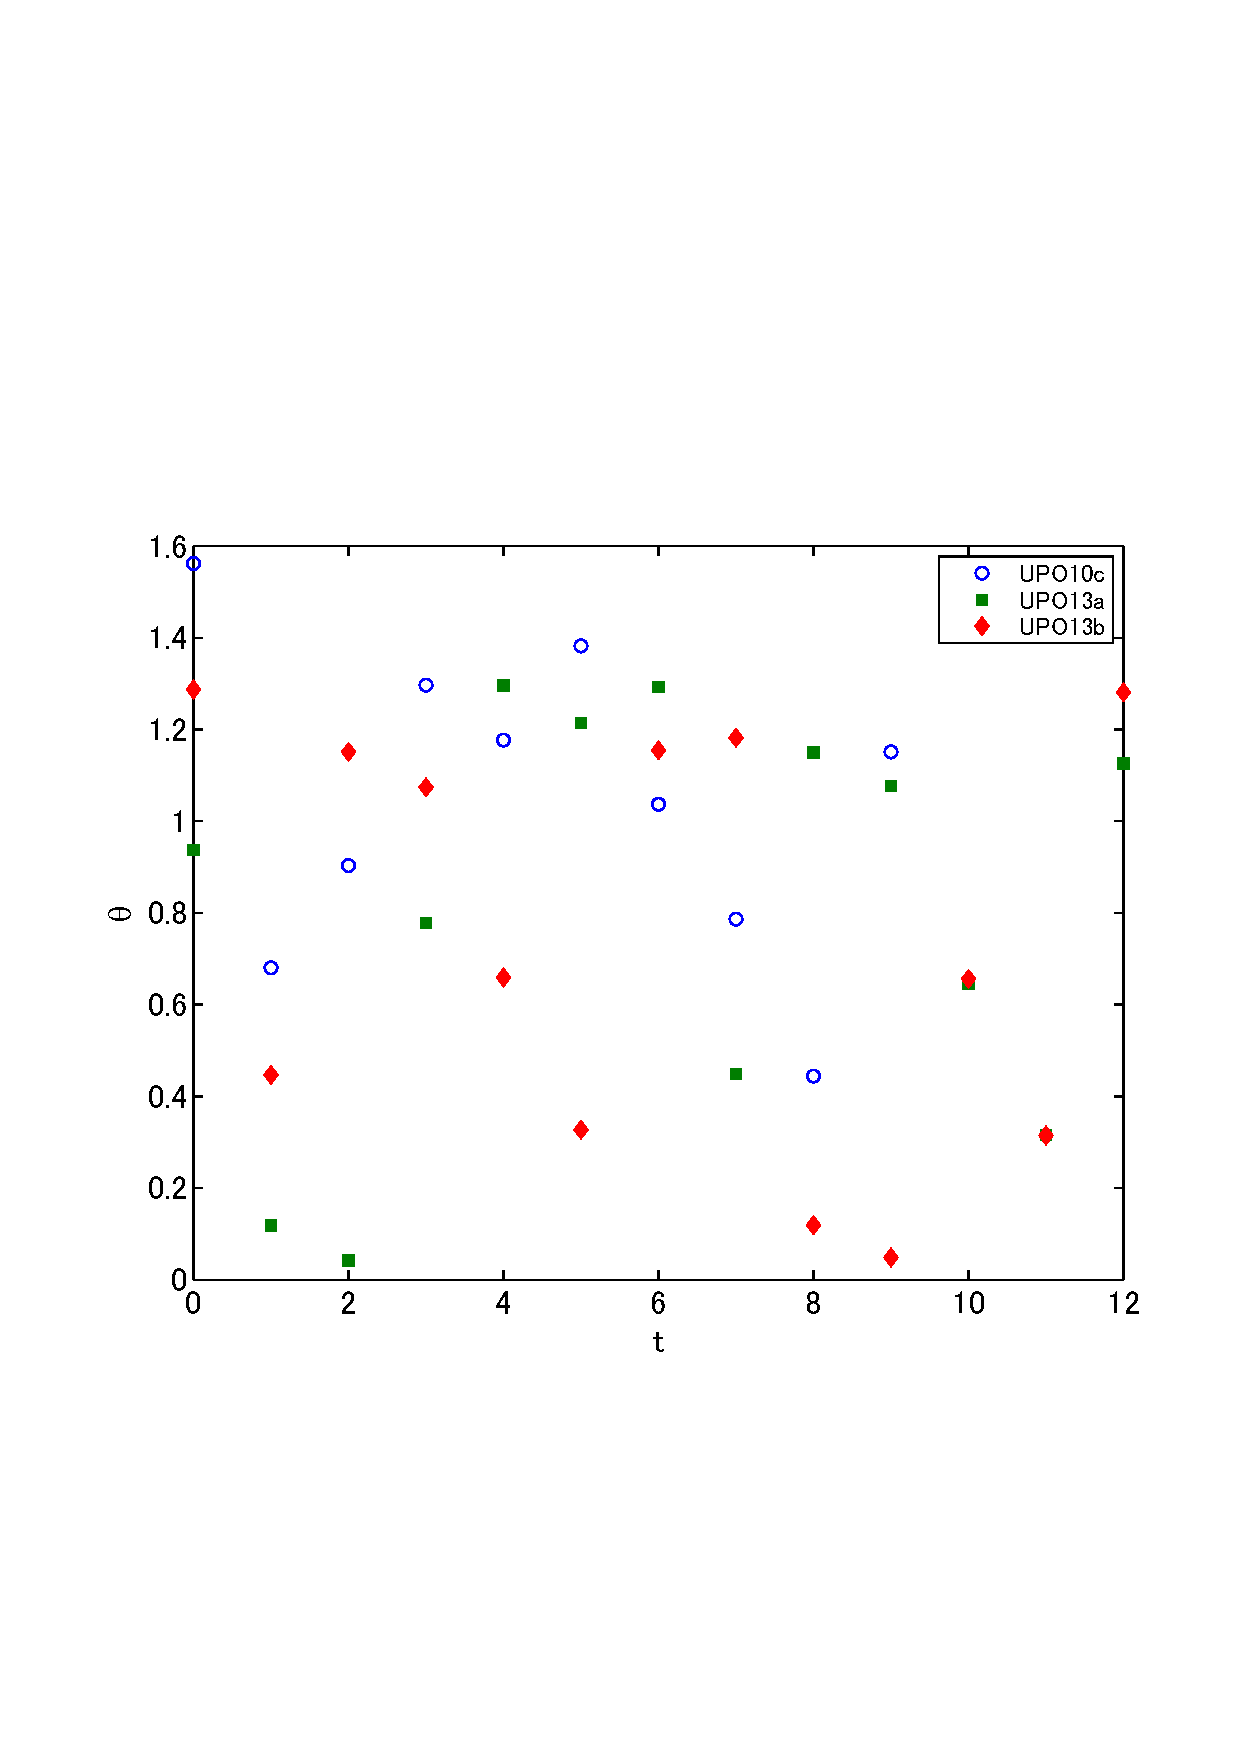
\includegraphics[width=0.45\textwidth]{fig1-hyperbolicity}
 (b)~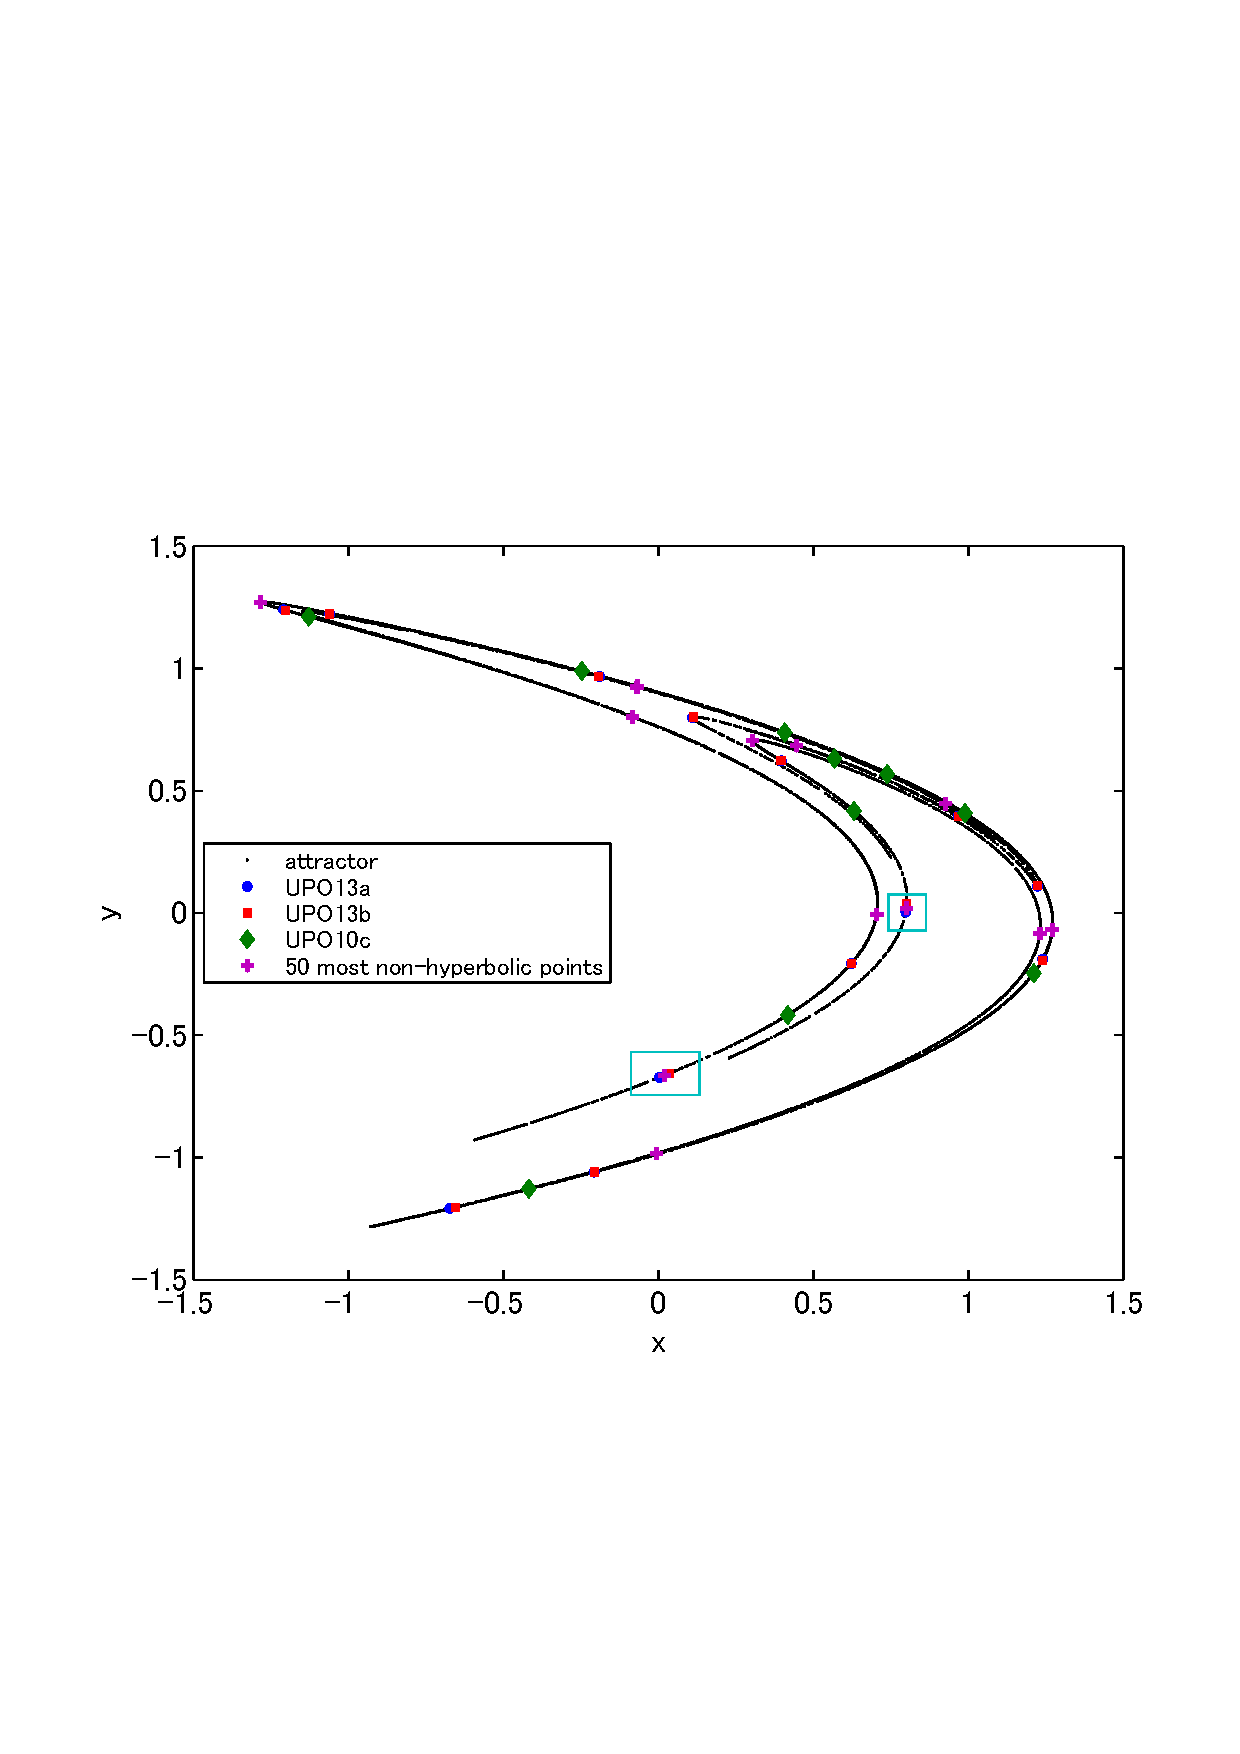
\includegraphics[width=0.45\textwidth]{fig2-nonhyp_points}
\caption{
(a)
(b)
[Kazz 2011-10-02].
}
\label{fig:HenonNonHypPoints}
\end{figure}

Here I use improved initial conditions for the UPOs and the results did
not change.

\refFig{fig:HenonNonHypPoints}\,(b) shows, on the top of the H\'enon attractor,
all the points of the above three UPOs (filled symbols, not the same ones
as \reffig{fig:HenonNonHypPoints}\,(a)) as well as the 50 most non-hyperbolic
points along a chaotic trajectory of length $10^6$ (plus symbols; most
non-hyperbolic means smallest angle here). We see that some of these
non-hyperbolic points are found very close to the non-hyperbolic UPOs
(see inside the light blue rectangles), while none of the non-hyperbolic
points are close to the hyperbolic UPO. However, we see that many
non-hyperbolic points are actually far enough from the two non-hyperbolic
UPOs, suggesting that there are other non-hyperbolic UPOs in this system.

\item[2011-10-03 Predrag] I do not remember other cycles being as
non-hyperbolic as these 13-cycles, but I should have a database of
thousands (?) of  H\'enon cycles somewhere, if you want to have a look...

\item[2011-08-09 Predrag] For comments to Takeuchi and Chat\'e\rf{TaCh11}
\emph{Can the inertial manifold be captured by unstable periodic
orbits?}, see [2011-07-21] entry, \refsect{sec:TaCh11}.

\item[2011-07-25 Kazz]
I am also a bit confused by not ordered time lines in the blog...

\item[2011-07-25 Predrag 2 Kazz]
Glad to oblige, but would be better if a question is answered pages
later, just because answer was typed at a later date? We who use subversion
always check the new edits using subversion diff, so we catch
edits anyplace in the blog...

\end{description}

\renewcommand{\ssp}{a}
